\documentclass[a4paper,12pt]{article}
\usepackage[utf8]{inputenc}
\usepackage[T1]{fontenc}
\usepackage{graphicx}
\usepackage{tabularx}
\usepackage{amsmath}
\usepackage{amssymb}
\usepackage{amsthm}
\usepackage{hyperref}
\usepackage{longtable}
\usepackage{color}
\usepackage{float}
\usepackage[backend=bibtex, style=numeric]{biblatex}
\addbibresource{citations.bib}
\usepackage{geometry}
\usepackage{kotex} % Korean language
\usepackage{lettrine} % large letter in start of paragraph
\usepackage{helvet}
\usepackage{caption}
\usepackage{subcaption}
\usepackage{enumitem}

\geometry{
	paper=a4paper, % Paper size
	top=2.5cm, % Top margin
	bottom=3cm, % Bottom margin
	left=2.5cm, % Left margin
	right=2.5cm, % Right margin
	headheight=25pt, % Header height
	footskip=1.5cm, % Space from the bottom margin to the baseline of the footer
	headsep=1cm, % Space from the top margin to the baseline of the header
	%showframe, % Uncomment to show how the type block is set on the page
}


\title{The Captaincy of ATEEZ: Steering Sound and Storytelling to Global Stardom}
\author{Jonas Werner\\ Matrikelnummer: 7987847}
\date{\today}

\usepackage{titling}

\setlength\droptitle {-38.5mm}
\renewcommand{\maketitlehooka}{%
\noindent\includegraphics[width=\linewidth]{images/ateez_logo_2.png}\par\vskip 3cm}%

\begin{document}
% Set Computer Modern Sans Serif (cmss) as the default font
\renewcommand{\rmdefault}{cmss}

\maketitle

\pagebreak
\tableofcontents

\vspace{2cm}

\begin{figure}[H]
    \centering
    \includegraphics[width=0.6\linewidth]{images/seonghwa_lego.jpg}
    \caption{\textit{ATEEZ}'s Seonghwa, proudly presenting his Legos!}
    \label{fig:enter-label}
\end{figure}

\pagebreak

\section{New Horizons}
\lettrine[lines=2]{\textit{ATEEZ}} \ (에이티즈) is a South Korean boy group formed rose to the top of the K-pop charts with their powerful performances, elegant stage presence, and a unique blend of music underlining their \hyperref[sec:backstory]{Pirate concept and Backstory}. Consisting of eight members—\hyperref[sec:memberhongjoong]{Hongjoong}, \hyperref[sec:memberseonghwa]{Seonghwa}, \hyperref[sec:memberyunho]{Yunho}, \hyperref[sec:memberyeosang]{Yeosang}, \hyperref[sec:membersan]{San}, \hyperref[sec:membermingi]{Mingi}, \hyperref[sec:memberwooyoung]{Wooyoung}, and \hyperref[sec:memberjongho]{Jongho}—the group gained international recognition and fame for their distinct sound, by combinin hip-hop, Rap, EDM, rock and R\&B. \textit{ATEEZ} is known for their iconic choreography, meaningful lyrics, and deep connection with \hyperref[sec:atiny]{ATINY}, the name of their fandom. \textit{ATEEZ} has shown to be one of the most influential groups of the fourth generation of K-pop, with a rapidly growing global fanbase.


\section{8 Makes One Team}
\textit{ATEEZ} consists of 8 members that each bring their unique talents and charm to the group. Their diverse personalities and skills make them an eye-catcher. Each member plays a unique role and holds a distinct position. In addition they are consistently listed in the same order, although not always appearing as such on photos.\\

\begin{figure}[h]
    \centering  % Centers the image
    \includegraphics[width=1\textwidth]{images/ateez_group.jpg}
    \caption{\textit{ATEEZ} 2019 with their 2nd Comeback \textit{Say my Name} \cite{ateez_saymyname}.\\ Left to right: Mingi, San, Yeosang, Hongjoong, Wooyoung, Yunho, Jongho, Seonghwa}
    \label{fig:ateezgroup}
\end{figure}

\subsection{Hongjoong (홍중)}\label{sec:memberhongjoong}
\textit{Hongjoong}, the leader or Captain, as he calls himself, of \textit{ATEEZ}, is known for his creativity and leadership skills. Born on November 7, 1998, he plays a key role in steering the group's musical direction by often contributing to songwriting and production. In addition, \textit{Hongjoong} shows a great sense of style and ability to captivate audiences with both his rap and stage presence, proving himself as the ideal Captain of the group. As the Captain, he not only guides the team but also ensures that each member has a voice.
\subsection{Seonghwa (성화)}\label{sec:memberseonghwa}
\textit{Seonghwa}, born on April 3, 1998, is known for his stunning visuals and versatile talent. He is one of the group's lead vocalists and is often admired for his powerful yet smooth and steady voice as well as his feminine energy. \textit{Seonghwa} has a unique ability to convey emotion through his singing which adds depth to \textit{ATEEZ}'s performances. Offstage, he is known for his shy, caring and thoughtful personality, immensely contrasting his monstrous and often dark stage presence. Thus Fans often refer to him as the Mother of \textit{ATEEZ} and together with \textit{Hongjoong}, \textit{Seonghwa} has a family of 6 which are the rest of the group.
\subsection{Yunho (윤호)}\label{sec:memberyunho}
\textit{Yunho}, born on March 23, 1999, is the group's lead dancer and vocalist. His exceptional dancing skills and high-energy performances have made him one of \textit{ATEEZ}'s standout performers. With his sharp choreography skills and powerful stage presence, \textit{Yunho} has a remarkable ability to command attention, setting him apart from the rest of the group. His playfulness also makes him a fan favorite, as he often brings a sense of joy and excitement to \textit{ATEEZ}'s interactions and fan-meetings with \textit{ATINY}.
\subsection{Yeosang (여상)}\label{sec:memberyeosang}
Yeosang, born on June 15, 1999, is a dancer and vocalist, known for his elegance. As one of the main dancers of ATEEZ, his ability to perform choreography with precision makes him an icon in the group’s performances. In addition to his dance skills, Yeosang’s smooth voice adds a layer of complexity to ATEEZ’s music. His calm and thoughtful nature provides aa contrast to the more energetic personalities of other members.
\subsection{San (산)}\label{sec:membersan}
\textit{San}, born on July 10, 1999, is known for his breath-taking energy including his athletic build and impressive vocal range. As one of ATEEZ's main vocalists, San's evolution from one of the thinnest to the one with the most incredible physique is something \textit{ATINY} admire a lot. He manages to deliver both powerful high notes and emotional low tones that make him an essential part of the dynamic of the group. His enthusiasm and dynamic stage presence have made him a standout figure in \textit{ATEEZ}'s performances, where he often captures the audience's attention with his captivating expressions.
\subsection{Mingi (민기)}\label{sec:membermingi}
\textit{Mingi}, born Augstu 9th 1999, is \textit{ATEEZ}'s main rapper, known for his deep voice. His unique rap stype features a powerful addition to the group. His performances are filled with passion. The Offstage-\textit{Mingi} is of very humerous and caring kind, demonstrating his special bond with the members and introducing some simple lightheartedness to the group.
\subsection{Wooyoung (우영)}\label{sec:memberwooyoung}
\textit{Wooyoung} was born on November 26th and  is the lead dancer and vocalist of the group. Known for his stunning visuals and amazing and stunning dancing, \textit{Wooyoung} contributes a lot of professionalism to \textit{ATEEZ}. \textit{Wooyoung} has a very joyful and upbeat personality, making him popular among \textit{ATINY} both on stage and during fan-meetings.
\subsection{Jongho (종호)}\label{sec:memberjongho}
\textit{Jongho}, borh on October 12, 2000, is the lead vocalist in \textit{ATEEZ}. Also being the youngest member of the group, \textit{Jongho} is often referred to as the \textit{Maknae}(막내). His breath-taking vocals and ability to crack apples in half without his voice trembling while being the yougest member of the group are the main reasons why \textit{Jongho} has been called the best 4th Generation vocalist in the K-Pop sector over and over again.

\section{A Journey With The Captain's Fellaz}\label{sec:history}
\subsection{Anchored at KQ}
KQ Entertainment, the agency behind \textit{ATEEZ} or Entertainment, as it is mostly referred to in the K-Pop industry, is a South-Korean company, founded by former \textit{JYP Enterntainment} Producer and Artist, \textit{Kim Kyu-wook}(김규욱) and quikly gained attention and presence in K-Pop, for fostering talent creating High-Quality music. The company is known for its innovative approach to approach to music production as well as artist development by placing a strong emphasis on creativity and innovation.

The small size and environment of KQ coupled with the overwhelming success of \textit{ATEEZ} demonstrates that success is possible without being one the three Giants (\textit{SM ENTERTAINMENT}, \textit{JYP ENTERTAINMENT} and \textit{HYBE LABELS}). It also gives \textit{ATEEZ} a unique character and charm that they likely wouldn't have developed had they debuted under a different, larger entertainment company. There have been, and continue to be, several successful groups and soloists who debuted under \textit{KQ}, including its most recent boy group, \textit{XIKERS}, which is already cultivating a global fanbase after having it's first . However, \textit{ATEEZ} remains the most prominent of them all.

\subsection{Story Of A Rookie Pirate}
Prior to \textit{ATEEZ}'s debut, the entertainment launched a Pre-Debut project known as \textit{KQ FELLAZ} which was a Pre-Debut Training-Group containing the Idols that would later be the members of \textit{ATEEZ}. The project fulfilled its purpose by promoting the company and the future idols, showcasing the members' individual talents. It allowed fans to familiarize themselves with their personalities, vocals, rap skills, and dance abilities before debut, laying a strong foundation and attracting thousands of loyal fans throughout it's initiative.

This careful pre-debut planning paid off, as \textit{ATEEZ} debuted with a strong and dedicated fanbase, eager to support the group’s journey. The \textit{KQ FELLAZ}'s exposure allowed fans to witness the chemistry between the members, laying the groundwork for \textit{ATEEZ}'s rise to stardom. \textit{KQ Entertainment}’s strategic approach to both artist development and fan engagement has been a key factor in ATEEZ’s success, as they were able to establish a sense of connection and loyalty with their audience from the very beginning, even before their initial debut, which is something not often witnessed with Rookie Groups.


\section{A Pirate's Story}\label{sec:backstory}
In their music videos, \textit{ATEEZ} conveys the conceptual narratives of a deep story which greatly exceeds what is shown in the music videos, immensely expanding upon and strengthening the meaning of their song lyrics and performances. The often called \textit{AU} or \textit{ATEEZ Universe} features a rich story with unique themes, adventures, rebellions, duality and pursuit of dreams. This story is told through music videos, song lyrics and additional content. The core complexity of self-development and resilience is delivered through metaphorical landscapes and unique character.

\subsection{The Treasure Series: Search for Freedom and Identity}
The Treasure Series is \textit{ATEEZ}'s debut arc and evolves around the idea of a treasure hunt. In this universe, the 8 members travel through adventurous dystopian worlds to find a hard-to grab treasure. This fleeting treasure is said to be the members' dreams, passion and sense for identity and symbolises the unversal human desire.\\

In their first music video \textit{"Pirate King"} \cite{ateez_pirateking}, the members are shown as modern pirates that travel through barren deserts and open seas. The picture telling and choreography show compasses, treasure maps and never-ending landscapes and underline \textit{ATEEZ}'s will to walk on their own path in an otherwhise unknown and hostile world. The sound and flow of the Song and album symbolise their rebellious spirit.\\

As the series progresses, songs like \textit{"Say My Name"} and \textit{"Hala Hala"} \cite{ateez_halahala} introduce darker tones and sounds. While \textit{"Say My Name"} symbolises courage, identity and the dream of recognition by inviting the listener to shout their name out loud, a figurative request of recognising \textit{ATEEZ}'s authenticity, \textit{"Hala Hala"} ilustrate societal expectations and personal doubt. In the music video, the members confront a group of eight masked men, symbolising repressed identities and individualities external presures, a recurring theme.\\

\textit{"Wave"} \cite{ateez_wave} and \textit{"Illusion"} \cite{ateez_illusion} bring a turning-point by showing moments of recovery and rest. The members are shown in a more lively manner, dreamlike scenarios, symbolising hope and companionship between the members. This heavy contrast tells the highs and lows of their journey and mirrors the real battle and struggle of following dreams.\\

\subsection{The Fever Series: Youth, Struggle and Duality}
ZERO: The \textit{Fever} series introduces an introspective and emotionally charged narrative. In this phase, \textit{ATEEZ} immerses itself int the complexity of Youth, passion and inner conflicts. The story shows immense contrasts such as light in the dark, hope and struggle and emphasizes the meaning of unity and self-conscience.\\

In \textit{"Inception"} \cite{ateez_inception} the borders between dream and reality mix and members appear trapped in surreal fragmented rooms. The repeating motive of fire symbolises both destruction and renewal, and reflects on their battle to overcome inner unrests in the search of inner purpose. This is further elaborated in the chapter \textit{"Answer"}, where the Group celebrates in ceremonial clothing their triumph, unity and adversity. The shadow visuals underlines their emotional duality.\\

\textit{"Thanxx"} \cite{ateez_thanxx} and \textit{"Deja Vu"} \cite{ateez_dejavu} expands upon this exploration of identity. \textit{"Thanxx"} rejects socialistic norms and expectations by adopting a rebellious tone. The lively visuals and unconventional backdrops represent their rejection of adapting to the societal norm while the lyrics emphasize to stay true to oneself. \textit{"Deja Vu"} is not at all like that, on the contrary. It shows the members trapped in a cycle of uncertainty and self-despair. This contradiction strongly reflects on the complexity of \textit{ATEEZ}'s emotions and struggle throughout the story of their journey.

\subsection{The World Series: Rebellion and Freedom}
\textit{The World} era which started with \textit{"Guerilla"} \cite{ateez_guerilla}, shows \textit{ATEEZ} in a new light. We once again can experience the freedom by fighting against the creativity and individuality-suppressing dystopia. \textit{The World} offers a wide variety blends of agressive energy and emotional depth. The possibly most well-known line \textit{"Break The Wall"} of the \textit{"Guerilla"} song lyrics are not only the climax in every concert, but also strongly symbolise the power that \textit{ATEEZ} holds to break down societal norms and destroy the dystopia they find themselves trapped inside of.

\vspace{2cm}
\begin{figure}[H]
    \centering
    \includegraphics[width=0.5\linewidth]{images/jongho_apple.jpg}
    \caption{\textit{ATEEZ}'s Jongho enjoying an Apple he just cracked while performing amazing high-notes}
    \label{fig:enter-label}
\end{figure}

\footnotetext[1]{Jongho is known for cracking open apples while singing intense high-notes without a crack in his voice \cite{ateezjonghoapplecracking}}

\newpage
\section{Treasure Hunt}
As of December 2024, \textit{ATEEZ} has released a total of 14 korean albums, 12 Mini- and 2 Full-Length albums, as well as 3 japanese albums and 10 singles. Their most significant releases are in this Album Art Mosaic:\\ \\

\begin{figure}[h]
    \centering  % Centers the image
    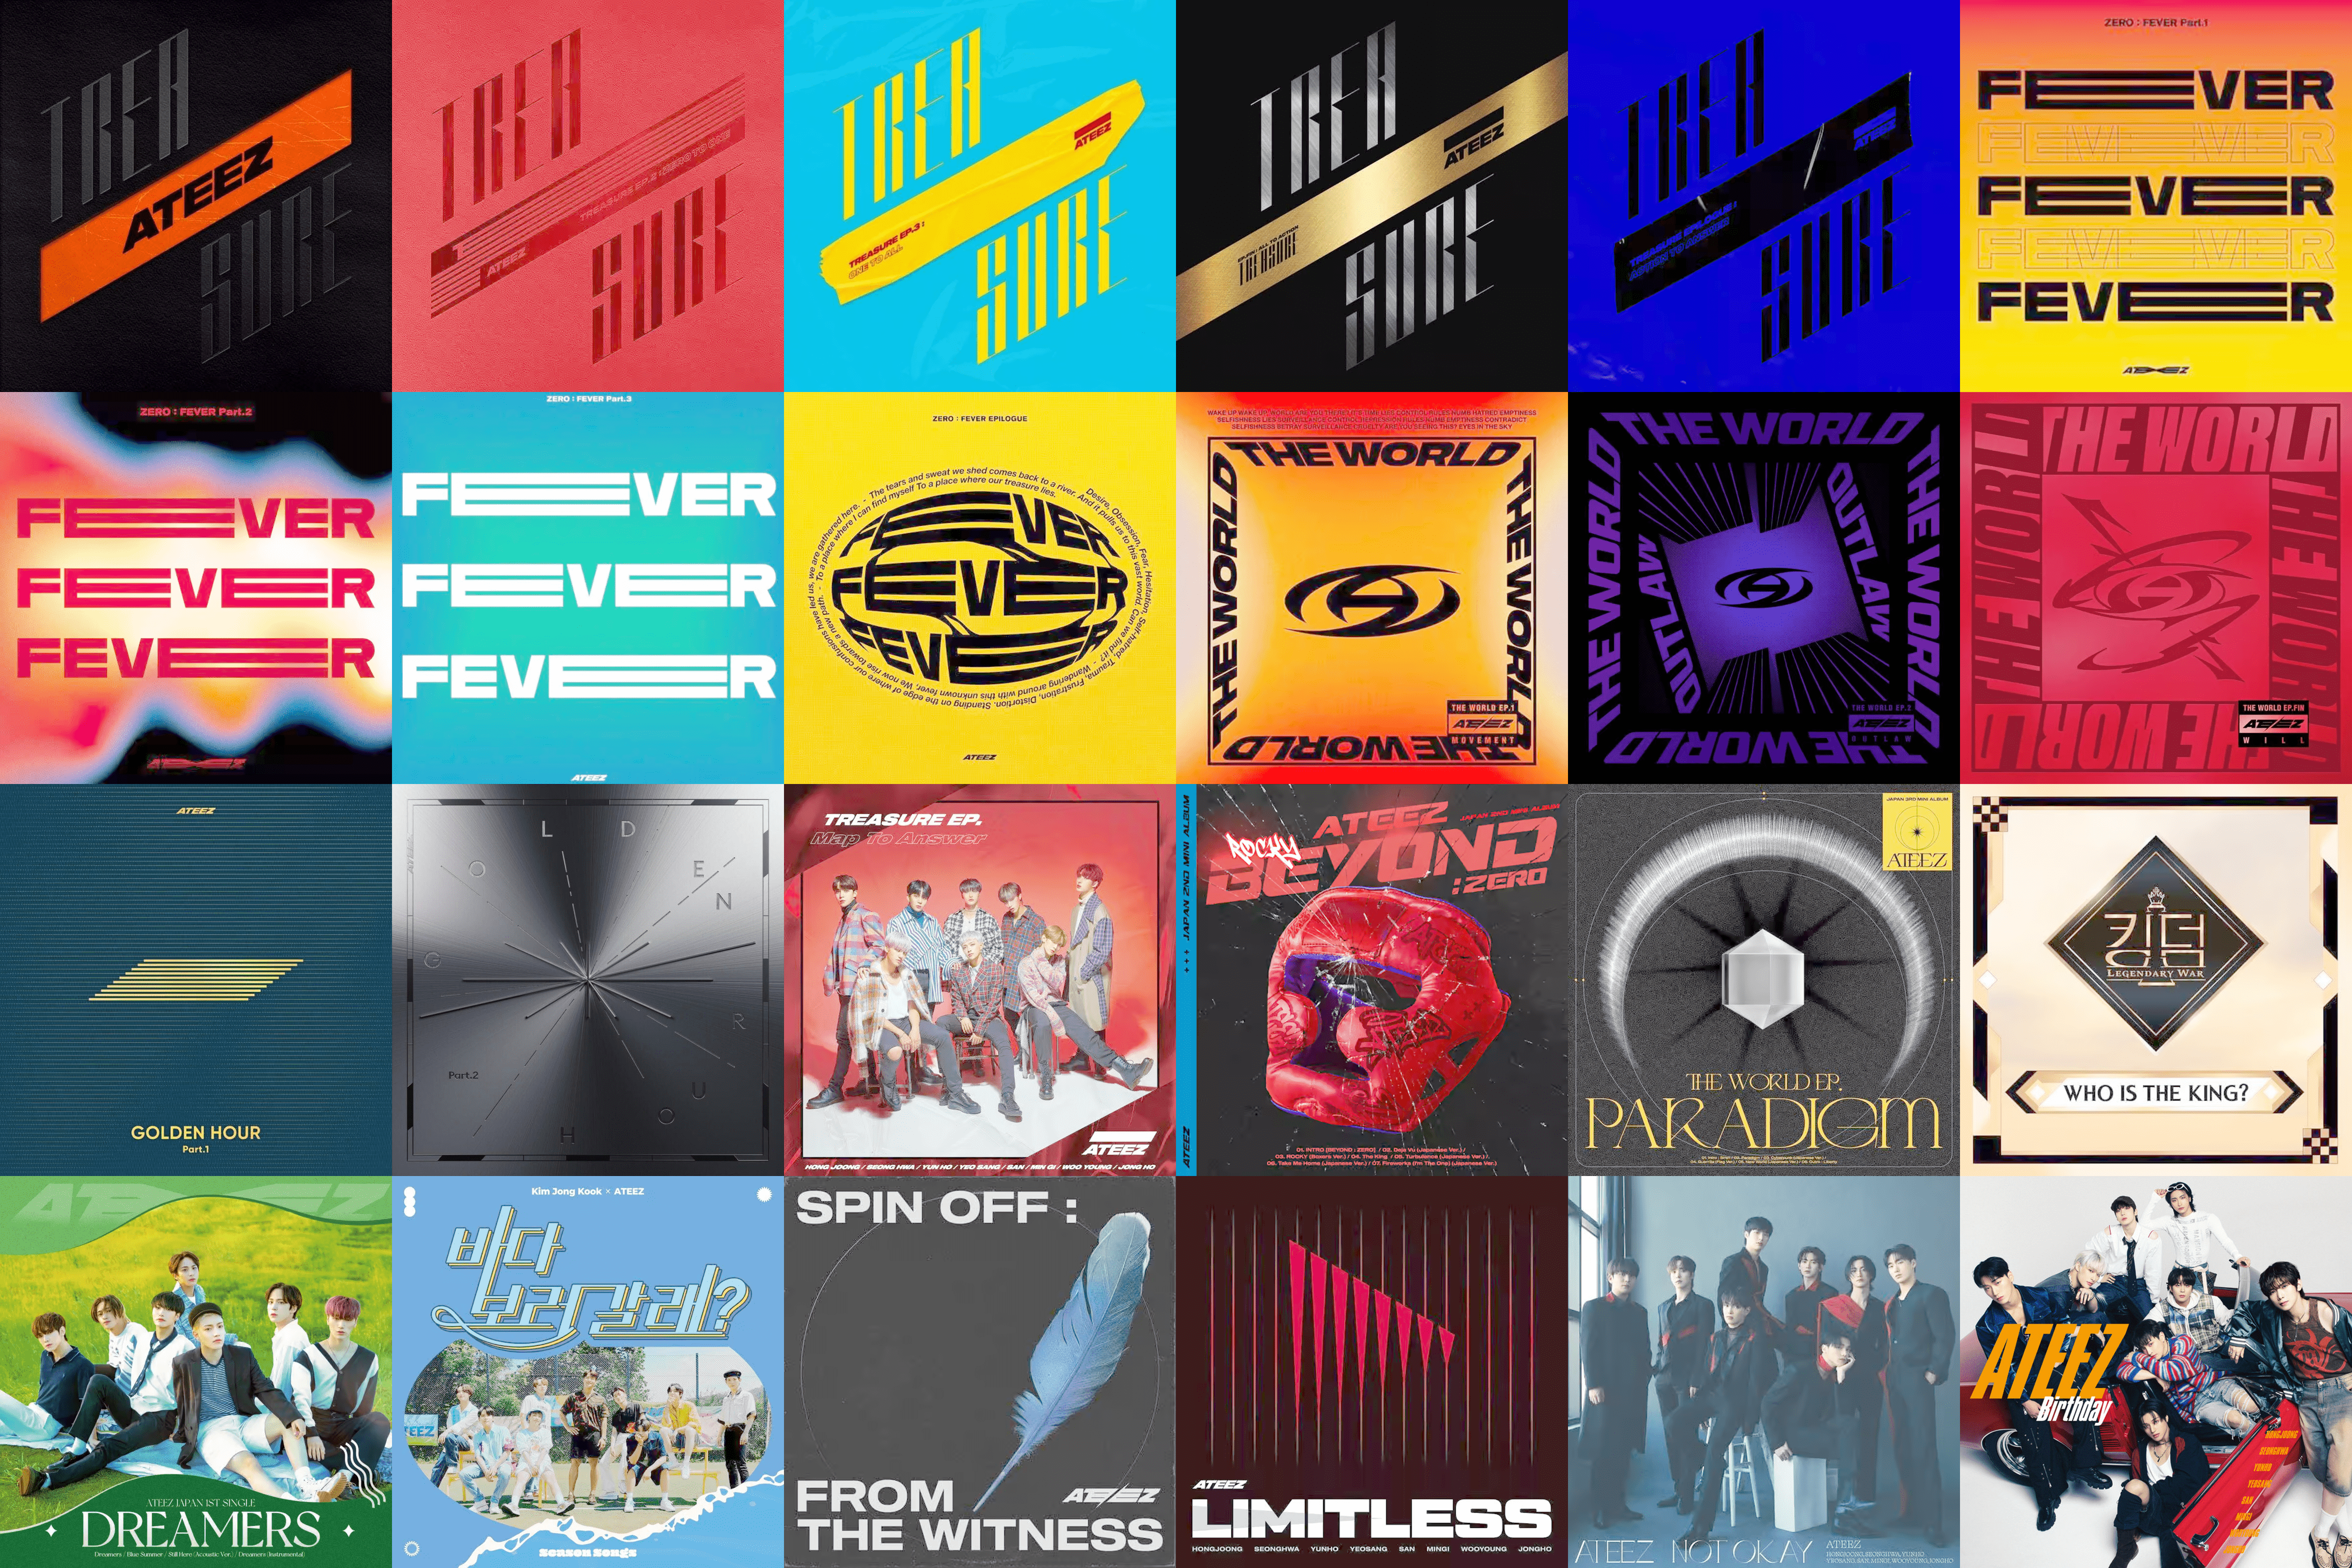
\includegraphics[width=1\textwidth]{images/ateez_albums.png}
    \caption{\textit{ATEEZ} most significant releases grouped by Korean Albums, Japanese Albums, Korean Singles and Japanese Singles sorted by release date in the order below}
    \label{fig:ateezgroup}
\end{figure}

These are:\\\\

\begin{table}[H]
\begin{tabularx}{\textwidth}{|X|r|}
    \hline
    Album Name & Release Date\\
    \hline
    TREASURE EP.1: All to Zero & October 24, 2018\\
    \hline
    TREASURE EP.2: Zero To One &  January 15, 2019\\
    \hline
    TREASURE EP.3: One To All &  June 10, 2019\\
    \hline
    TREASURE EP.FIN: All To Action & October 8, 2019\\
    \hline
    TREASURE EPILOGUE : Action To Answer & January 6, 2020\\
    \hline
    ZERO : FEVER Part.1 & July 29, 2020\\
    \hline
    ZERO : FEVER Part.2 & March 1, 2021\\
    \hline
    ZERO : FEVER Part.3 & September 13, 2021\\
    \hline
    ZERO : FEVER EPILOGUE & December 10, 2021\\
    \hline
    THE WORLD EP.1 : MOVEMENT &  July 29, 2022\\
    \hline
    THE WORLD EP.2 : OUTLAW & June 16, 2023\\
    \hline
    THE WORLD EP.FIN : WILL & December 1, 2023\\
    \hline
    GOLDEN HOUR : Part.1 & May 31, 2024\\
    \hline
    GOLDEN HOUR : Part.2 & November 15, 2024\\
    \hline
\end{tabularx}
\caption{\textit{ATEEZ} Korean albums}
\end{table}

\begin{table}[H]
\begin{tabularx}{\textwidth}{|X|r|}
    \hline
    Album Name & Release Date\\
    \hline
    TREASURE EP. Map To Answer & February 12, 2020\\
    \hline
    BEYOND : ZERO &  May 25, 2022\\
    \hline
    THE WORLD EP.PARADIGM &  November 30, 2022\\
    \hline
\end{tabularx}
\caption{\textit{ATEEZ} Japanese albums}
\end{table}

\begin{table}[H]
\begin{tabularx}{\textwidth}{|X|r|}
    \hline
    Album Name & Release Date\\
    \hline
    킹덤 KINGDOM <FINAL : WHO IS THE KING?> & May 28, 2021\\
    \hline
    Dreamers &  July 28, 2021\\
    \hline
    Season Songs &  August 16, 2021\\
    \hline
    SPIN OFF : FROM THE WITNESS & December 30, 2022\\
    \hline
    Limitless & March 22, 2023\\
    \hline
    NOT OKAY & February 28, 2024\\
    \hline
    Birthday & October 2, 2024\\
    \hline
\end{tabularx}
\caption{\textit{ATEEZ} Korean and Japanese singles}
\end{table}


\newpage
\section{Global Piracy}\label{sec:atiny}
\textit{ATINY}, the official Fandom name of \textit{ATEEZ}, is an essential part of their success and identity. The name is a combination of the group name and \textit{"Destiny"}.

\subsection{Pirate Havens}
\textit{ATEEZ} has been on many World Tours where they have played concerts in many different citites globally. Their most significant Tours are:\\
\begin{enumerate}
    \item The Expedition Tour (2019)
    \item The Fellowship: Beginning of the End (2022)
    \item The Fellowship: Break The Wall (2023/2024)
\end{enumerate}
The group is currently on tour and the upcoming Europe Tour is next year:\\
\begin{enumerate}[start=4]
    \item Towards The Light: Will To Power (2024/2025)
\end{enumerate}


\subsection{A Pirate's light}
Like many other groups, \textit{ATEEZ} has an official Fanlight/Lighstick, that \textit{ATINY} are encouraged to bring to the concerts. \textit{LIGHTINY 2}, the current \textit{ATEEZ} lighstick, syncs with the stage lights to the beat of the music and makes the concerts even more magical. They are an essential part of \textit{ATEEZ}'s merch and most \textit{ATINY} own one.\\

\begin{figure}[H]
  \begin{subfigure}[t]{0.3\textwidth}
    \includegraphics[width=\textwidth]{images/ateez_lighsticks.jpg}
    \caption{Me (Right) and two friends of mine at an \textit{ATEEZ} concert with our Lightsticks.}
    \label{fig:lightsticks_us}
  \end{subfigure}
  \hfill
  \begin{subfigure}[t]{0.6\textwidth}
    \includegraphics[width=\textwidth]{images/ateez_lighsticks_concert.jpg}
    \caption{A couple thousand Lighsticks at a concert.}
    \label{fig:f2}
  \end{subfigure}
  \caption{K-Pop Lighsticks}
\end{figure}

\section{Finding The Treasure}
Such enormous success doesn't come without awards! Over the years \textit{ATEEZ} has earned numerous awards and chart milestones. They have won wards like the \textit{Golden Music Awards} and \textit{Billboard's} World Albums Charts. Below is a list of all relevant achievements since the group's debut \cite{ateezwiki} \cite{ateezawards}:\\

\begin{itemize}
    \item 2019:
    \begin{itemize}
        \item MAMA Awards: Worldwide Fans’ Choice Top 10
        \item MTV Europe Music Awards: Best Korean Act
        \item Mubeat Awards: Best Song \textit{“WONDERLAND”}
        \item Soribada Best K-Music Awards: Performance Award
    \end{itemize}
    \item 2020:
    \begin{itemize}
        \item Asia Model Awards: Popular Star Award – Male Singer
        \item Golden Disc Awards: Next Generation Award
        \item MAMA Awards: Worldwide Fans’ Choice Top 10, Discovery of the Year
        \item The Fact Music Awards: Global Hottest Artist
    \end{itemize}
    \item 2021:
    \begin{itemize}
        \item Gaon Chart Music Awards: World Rookie of the Year
        \item Hanteo Music Awards: Initial Chodong Record Award
        \item Seoul Music Awards: Main Award (Bonsang)
        \item The Fact Music Awards: Artist of the Year (Bonsang)
    \end{itemize}
    \item 2022:
    \begin{itemize}
        \item Forbes Korea Awards: The Best Fandom
        \item Seoul Music Awards: Main Award (Bonsang)
        \item The Fact Music Awards: Artist of the Year (Bonsang), Best Performer
    \end{itemize}
    \item 2023:
    \begin{itemize}
        \item K Global Heart Dream Awards: K Global Best World Tour Award, K Global Bonsang (Main Prize)
        \item MAMA Awards: Worldwide Fans’ Choice Top 10, Favorite Global Performer – Male Group
        \item The Fact Music Awards: Artist of the Year (Bonsang)
    \end{itemize}
    \item 2024:
    \begin{itemize}
        \item iHeartRadio Music Awards: K-pop Song of the Year, Best Fan Army
        \item Korea Grand Music Awards: Best Song, Grand Honor's Choice (Daesang)
        \item MAMA Awards: Album of the Year, Worldwide Fans' Choice Top 10
        \item Melon Music Awards: Global Artist - Male
    \end{itemize}
\end{itemize}

\newpage
\section{And now for something completely different: Etwas Mathe zwischendurch}
Die folgende Herleitung wird dadurch besonders schön und übersichtlich, dass alle Gleichheitszeichen und alle Kommentare/Rechenschritte jeweils untereinander angeordnet sind und dadurch, dass die Klammern und Wurzelzeichen passende Größen haben:\\
\[
\begin{aligned}
    0 &= x^2 + px + q  &&\quad \text{| } + \left(\frac{p^2}{4} - \frac{p^2}{4} = 0\right) \\
    0 &= x^2 + px + \frac{p^2}{4} + q - \frac{p^2}{4}  &&\quad \text{Potenzgesetz} \\
    0 &= x^2 + px + \left(\frac{p}{2}\right)^2 + q - \frac{p^2}{4} &&\quad \text{Binomische Formel} \\
    0 &= \left(x + \frac{p}{2}\right)^2 + q - \frac{p^2}{4} &&\quad \text{| } - q + \frac{p^2}{4} \\
    \frac{p^2}{4} - q &= \left(x + \frac{p}{2}\right) &&\quad \text{| } \sqrt{\phantom{x}}\\
    \pm \sqrt{\frac{p^2}{4} - q} &= x + \frac{p}{2} &&\quad \text{| } - \frac{p}{2}\text{; L.S. $\Leftrightarrow$ R.S.}\\
    x &= - \frac{p}{2} \pm \sqrt{\frac{p^2}{4} - q}
\end{aligned}
\]\\
Für die folgenden Summen wurde ein eigener Befehl \verb|\bs| mit Argumenten für den Summationsindex, den Beginn, das Ende und die Basis, also instgesamt vier, definiert und verwendet:\\

\newcommand{\bs}[4]{\sum\limits_{\substack{#1=#2}}^{#3} #4}

\[
\begin{aligned}
&\bs{i}{1}{n}{(2 \cdot i - 1)} = n^2 \quad&&\quad \bs{k}{2}{4}{2^k} = 28 \\
&\bs{j}{0}{1}{q^j} = \frac{1 - q^{n + 1}}{1 - q} \quad&&\quad \bs{i}{0}{\infty}{\left(\frac{1}{4}\right)^i} = \frac{1}{1 - \frac{1}{4}} = \frac{4}{3} = 1,\overline{3} \\
\end{aligned}
\]\\
Die Summenfunktion $f: \mathbb{N} \rightarrow \mathbb{N}$ ist definiert als:\\
\[f(n)=\begin{cases}
        0 & \text{falls } n = 0\\
        n + f(n - 1) & \text{sonst.}\\
\end{cases}\]\\

Zum Abschluss noch ein paar Zeichen, deren Befehle rauszusuchen waren:\\
\[\mathcal{P}, \varphi, \phi, \binom{n}{k}, \in, \neg, \wedge, \vee, \oplus, \cap\]

\printbibliography
\listoffigures
\listoftables

\end{document}
